\documentclass[journal,12pt,twocolumn]{IEEEtran}

\usepackage{setspace}
\usepackage{gensymb}
\singlespacing
\usepackage[cmex10]{amsmath}

\usepackage{amsthm}

\usepackage{mathrsfs}
\usepackage{txfonts}
\usepackage{stfloats}
\usepackage{bm}
\usepackage{cite}
\usepackage{cases}
\usepackage{subfig}

\usepackage{longtable}
\usepackage{multirow}

\usepackage{enumitem}
\usepackage{mathtools}
\usepackage{steinmetz}
\usepackage{tikz}
\usepackage{circuitikz}
\usepackage{verbatim}
\usepackage{tfrupee}
\usepackage[breaklinks=true]{hyperref}
\usepackage{graphicx}
\usepackage{tkz-euclide}

\usetikzlibrary{calc,math}
\usepackage{listings}
    \usepackage{color}                                            %%
    \usepackage{array}                                            %%
    \usepackage{longtable}                                        %%
    \usepackage{calc}                                             %%
    \usepackage{multirow}                                         %%
    \usepackage{hhline}                                           %%
    \usepackage{ifthen}                                           %%
    \usepackage{lscape}     
\usepackage{multicol}
\usepackage{chngcntr}

\DeclareMathOperator*{\Res}{Res}

\renewcommand\thesection{\arabic{section}}
\renewcommand\thesubsection{\thesection.\arabic{subsection}}
\renewcommand\thesubsubsection{\thesubsection.\arabic{subsubsection}}

\renewcommand\thesectiondis{\arabic{section}}
\renewcommand\thesubsectiondis{\thesectiondis.\arabic{subsection}}
\renewcommand\thesubsubsectiondis{\thesubsectiondis.\arabic{subsubsection}}


\hyphenation{op-tical net-works semi-conduc-tor}
\def\inputGnumericTable{}                                 %%

\lstset{
%language=C,
frame=single, 
breaklines=true,
columns=fullflexible
}
\begin{document}

\newcommand{\BEQA}{\begin{eqnarray}}
\newcommand{\EEQA}{\end{eqnarray}}
\newcommand{\define}{\stackrel{\triangle}{=}}
\bibliographystyle{IEEEtran}
\raggedbottom
\setlength{\parindent}{0pt}
\providecommand{\mbf}{\mathbf}
\providecommand{\pr}[1]{\ensuremath{\Pr\left(#1\right)}}
\providecommand{\qfunc}[1]{\ensuremath{Q\left(#1\right)}}
\providecommand{\sbrak}[1]{\ensuremath{{}\left[#1\right]}}
\providecommand{\lsbrak}[1]{\ensuremath{{}\left[#1\right.}}
\providecommand{\rsbrak}[1]{\ensuremath{{}\left.#1\right]}}
\providecommand{\brak}[1]{\ensuremath{\left(#1\right)}}
\providecommand{\lbrak}[1]{\ensuremath{\left(#1\right.}}
\providecommand{\rbrak}[1]{\ensuremath{\left.#1\right)}}
\providecommand{\cbrak}[1]{\ensuremath{\left\{#1\right\}}}
\providecommand{\lcbrak}[1]{\ensuremath{\left\{#1\right.}}
\providecommand{\rcbrak}[1]{\ensuremath{\left.#1\right\}}}
\theoremstyle{remark}
\newtheorem{rem}{Remark}
\newcommand{\sgn}{\mathop{\mathrm{sgn}}}
\providecommand{\abs}[1]{\vert#1\vert}
\providecommand{\res}[1]{\Res\displaylimits_{#1}} 
\providecommand{\norm}[1]{\lVert#1\rVert}
%\providecommand{\norm}[1]{\lVert#1\rVert}
\providecommand{\mtx}[1]{\mathbf{#1}}
\providecommand{\mean}[1]{E[ #1 ]}
\providecommand{\fourier}{\overset{\mathcal{F}}{ \rightleftharpoons}}
%\providecommand{\hilbert}{\overset{\mathcal{H}}{ \rightleftharpoons}}
\providecommand{\system}{\overset{\mathcal{H}}{ \longleftrightarrow}}
	%\newcommand{\solution}[2]{\textbf{Solution:}{#1}}
\newcommand{\solution}{\noindent \textbf{Solution: }}
\newcommand{\cosec}{\,\text{cosec}\,}
\providecommand{\dec}[2]{\ensuremath{\overset{#1}{\underset{#2}{\gtrless}}}}
\newcommand{\myvec}[1]{\ensuremath{\begin{pmatrix}#1\end{pmatrix}}}
\newcommand{\mydet}[1]{\ensuremath{\begin{vmatrix}#1\end{vmatrix}}}
\numberwithin{equation}{subsection}
\makeatletter
\@addtoreset{figure}{problem}
\makeatother
\let\StandardTheFigure\thefigure
\let\vec\mathbf
\renewcommand{\thefigure}{\theproblem}
\def\putbox#1#2#3{\makebox[0in][l]{\makebox[#1][l]{}\raisebox{\baselineskip}[0in][0in]{\raisebox{#2}[0in][0in]{#3}}}}
     \def\rightbox#1{\makebox[0in][r]{#1}}
     \def\centbox#1{\makebox[0in]{#1}}
     \def\topbox#1{\raisebox{-\baselineskip}[0in][0in]{#1}}
     \def\midbox#1{\raisebox{-0.5\baselineskip}[0in][0in]{#1}}
\vspace{3cm}
\title{AI1103-Assignment 4}
\author{Name : Ayush Jha \\ Roll Number: CS20BTECH11006}
\maketitle
\newpage
\bigskip
\renewcommand{\thefigure}{\theenumi}
\renewcommand{\thetable}{\theenumi}
Download all python codes from 
\begin{lstlisting}
https://github.com/ayushjha2612/AI11003/tree/main/Assignment4/Codes
\end{lstlisting}
%
and latex-tikz codes from 
%
\begin{lstlisting}
https://github.com/ayushjha2612/AI11003/tree/main/Assignment4
\end{lstlisting}
\section*{GATE 2017 (XE-A), Q.170}
Two dice are thrown simultaneously. The probability that the product of the numbers appearing on the top faces of the dice is a perfect square is  \\ \\
(A)$\dfrac{1}{9}$         \hfill  (B) $\dfrac{2}{9}$  \hfill
(C)$\dfrac{1}{3}$      \hfill       (D)$\dfrac{4}{9}$  
\section*{Answer}
Option (B) $\dfrac{2}{9}$
\section*{Solution}
Let X be a random variable which is equal to 1, when the product of the numbers appearing on the top faces of the dice is a perfect square and 0 when it is not a perfect square. \\
The total no. of possible outcomes is 36.\\
Outcomes corresponding to $ X =1 $ are listed in table \ref{tab:Outcomes}
\begin{table}[hbt!]
\centering
\begin{tabular}{|c|c|}
\hline
\textbf{Squares} & \textbf{Favourable outcomes} \\ \hline
1                & (1,1)                        \\ \hline
4                & (1,4) , (2,2) , (4,1)        \\ \hline
9                & (3,3)                        \\ \hline
16               & (4,4)                        \\ \hline
25               & (5,5)                        \\ \hline
36               & (6,6)                        \\ \hline
\end{tabular}
\caption{Outcomes for X=1}
\label{tab:Outcomes}
\end{table}
The total no. of favourable outcomes are 8. Therefore we have,
\begin{align}
    \Pr\brak{X=1}    &= \dfrac{8}{36}  \\
     &= \dfrac{2}{9}
\end{align}
Similarly we have that the probability of not getting a perfect square as a product i.e. $X=0$
\begin{align}
    \Pr\brak{X=0} & = 1-  \Pr\brak{X=1} \\
    &=  1-\dfrac{2}{9}  \\
     &= \dfrac{7}{9}
\end{align}
The simulation vs analysis plot can be seen at figure  \ref{Probability distribution}. Simulations are close to analysis\\
Therefore the probability that the product of the numbers appearing on the top faces of the dice is a perfect square is $\frac{2}{9}$  i.e. option (B).

\begin{figure}[h!]
    \centering
    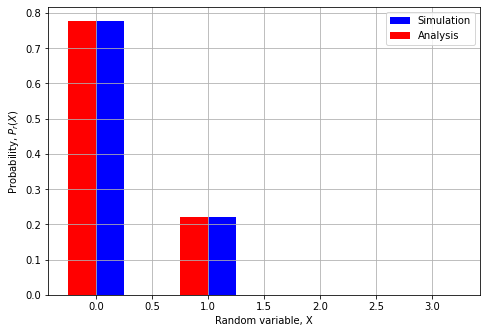
\includegraphics[width=.9\columnwidth]{Assignment_4.png}
    \caption{Probability distribution of X}
    \label{Probability distribution}
\end{figure}
\end{document}